\documentclass[12pt]{article}
\usepackage[paper=a4paper, margin=1in]{geometry} 

%Required packages
\usepackage{natbib} 
\usepackage{graphicx}
\usepackage{amsmath}
\usepackage{mathtools}
\usepackage{setspace}
\usepackage[document]{ragged2e}
\usepackage{lineno}
\usepackage{gensymb}
\setcounter{secnumdepth}{-1} 
\raggedright

\title{Supplementary Material for: \\
What controls the range of hosts a fish parasite infects?}

\author{Tad Dallas$^{1,2}$, Andrew Park $^{1}$, and John M. Drake$^{1}$}

\begin{document}
 

\maketitle{}

\section{Does parasite taxonomy or host specificity influence predictive accuracy?}

No, not really. 







\section{Figures}
\begin{figure}[h]
  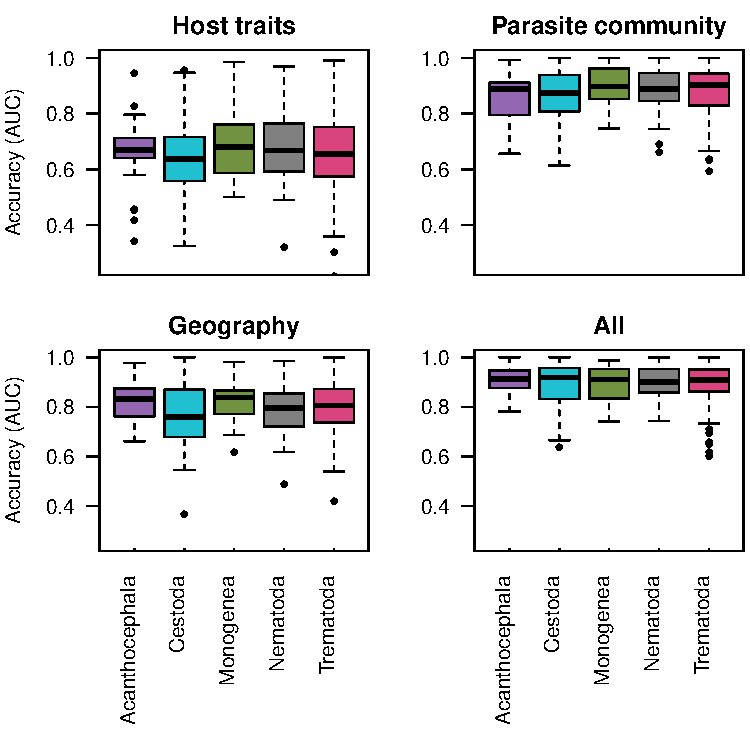
\includegraphics[width=\textwidth]{../Figures/parAccuracy.pdf}
  \caption{Accuracy (Area under Receiver operating characteristic (ROC) curves) for boosted regression models trained using host traits (top left), parasite community similarity (top right), geographic variables (bottom left), and all available data (bottom right) as a function of parasite type ($x$-axis).   }
 \label{fig:parAUC}
 \end{figure}

 
  
 
 \newpage
 \begin{figure}[h!]
  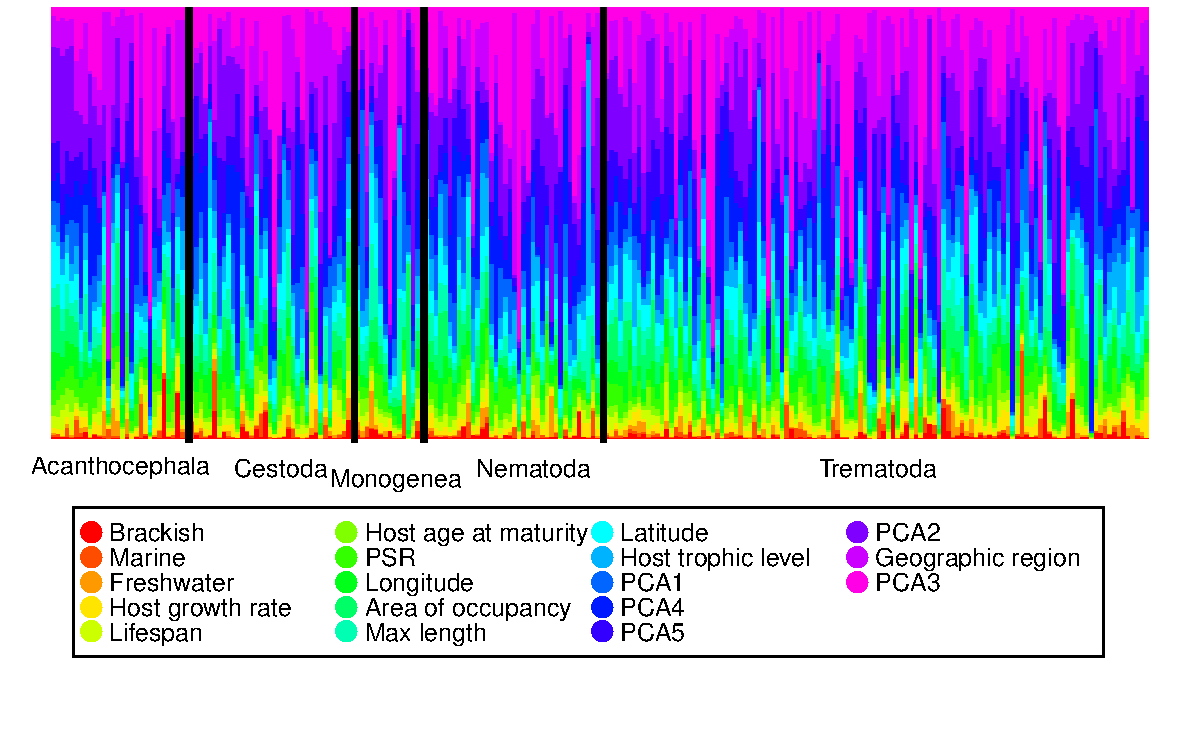
\includegraphics[width=\textwidth]{../Figures/parTypeColor.pdf}
  \caption{Variation in variable importance as a function of parasite type. Each column represents a model trained on occurrence data for a single parasite species. Variables are sorted by their mean relative importance values across parasite species, but these values vary among parasite species.}
 \label{fig:parType}
 \end{figure}


 
 
\begin{figure}[h]
  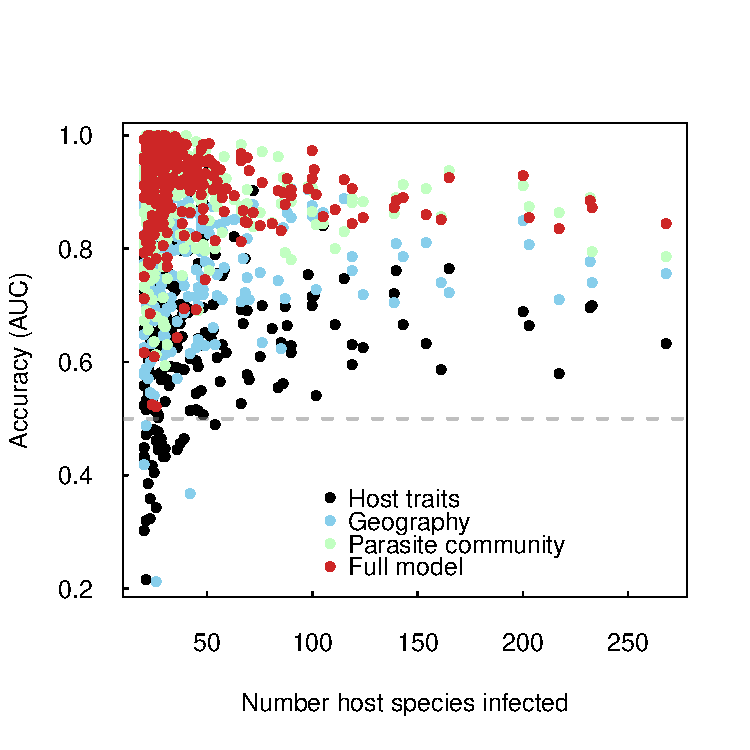
\includegraphics[width=\textwidth]{../Figures/hostNumAccuracy.pdf}
  \caption{Accuracy (Area under Receiver operating characteristic (ROC) curves) for boosted regression models trained using host traits, parasite community similarity, geographic variables, and all available data as a function of the number of hosts the parasite species was collected on ($x$-axis). This host range estimate was uncorrelated to accuracy, though some models trained on host traits (black dots) performed poorly when parasite species were specific to a smaller number of host species. }
 \label{fig:HostNum}
 \end{figure}

 
 
 \end{document}